\setlength{\footskip}{8mm}
% \setstretch{1}

\chapter{Results and Discussion}
\label{ch:results}

\textit{In this chapter, the outcome of the evaluation tests are shown. Firstly, the necessary preliminary conditions are outlined. Then the actual test results according to the desired parameters are detailed and discussed on.}

\section{Preliminary Conditions}
\label{sect:preconditions}
In order to carry out a successful experiment, some necessary pre-conditions need to be observed. These are stated as follows.

\begin{enumerate}
  \item The drone needs to have sufficient battery for a full flight, as it will not be able to arm and takeoff if its detected battery level is below the failsafe threshold. The minimum starting battery level is around 60\% although a full battery is always recommended.
  \item The drone has to be turned on at a clear location for it to obtain a GPS lock, as it will not arm without a lock.
  \item All hardware has to be fully functional.
\end{enumerate}

\section{Experimental Environment and Results}
The test mission consists of a delivery mission type to the northwestern corner of the AIT main football field. The drone takes off from the southwestern corner of the field. The flights are carried out by the drone consecutively. The summarized results are shown in Table \ref{table:allresults} and the evaluation parameters are discussed in the subsequent sections.

% \begin{table}[t]
%   \linespread{0.6}\selectfont
%   \renewcommand{\arraystretch}{1.5}
%   \caption{\small Experimental Results.}
%   \begin{center}
%     \begin{tabu} to \textwidth {| X[c] | X[c] | X[c] | X[c] |}
%       \hline \textbf{Flight number} & \multicolumn{2}{|c|}{\textbf{Total flight time}} & \multicolumn{2}{|c|}{\textbf{Reliability}}  & \textbf{Estimated landing error margin (cm)}\\ \hline
%       & \textbf{Simulator} & \textbf{Drone} & \textbf{Outcome }& \textbf{Cause} & \\ [10pt] \hline
%       Flight 1 & 3 minutes 1 second & 0 minutes 24 seconds & Failure &  Uncalibrated weight causing wrong thrust & N/A\\ [10pt] \hline
%       Flight 2 & 2 minutes 53 seconds  & 2 minutes 59 seconds & Successful & - & 160cm\\ [10pt] \hline
%       Flight 3 & 2 minutes 51 seconds & 3 minutes 1 second & Successful & - & 30cm\\ [10pt] \hline 
%       Flight 4 & 2 minutes 58 seconds & 1 minutes 12 seconds & Successful but terminated & Demonstration of mission parameter change & 90cm\\ [10pt] \hline
%       Flight 5 & 2 minutes 53 seconds & 1 minutes 51 seconds & Failure & Depleted battery and crashed & N/A\\ [10pt] \hline
%     \end{tabu}
%   \end{center}
%   \label{table:allresults}
% \end{table}
% \FloatBarrier

\begin{table}[t]
  \linespread{0.6}\selectfont
  \renewcommand{\arraystretch}{1.5}
  \caption{Experimental results.}
  \begin{center}
    \begin{tabu} to \textwidth {| X[c] | X[c] | X[c] | X[c] | X[c] |}
      \hline \textbf{Flight number} & \textbf{Total flight time (simulator)} & \textbf{Total flight time (real drone)} & \textbf{Reliability}  & \textbf{Estimated landing error margin (cm)}\\ \hline \hline
      Flight 1 & 3 minutes 1 second & 0 minutes 24 seconds &  Failure due to uncalibrated weight causing wrong thrust & N/A\\ [10pt] \hline
      Flight 2 & 2 minutes 53 seconds  & 2 minutes 59 seconds & Successful & 160cm\\ [10pt] \hline
      Flight 3 & 2 minutes 51 seconds & 3 minutes 1 second & Successful & 30cm\\ [10pt] \hline 
      Flight 4 & 2 minutes 58 seconds & 1 minutes 12 seconds & Successful but terminated & 90cm\\ [10pt] \hline
      Flight 5 & 2 minutes 53 seconds & 1 minutes 51 seconds & Failure due to depleted battery and crashed & N/A\\ [10pt] \hline
    \end{tabu}
  \end{center}
  \label{table:allresults}
\end{table}
\FloatBarrier

% \begin{table}[t]
%   \caption{\small Experimental Results.}
%   \begin{center}
%     \begin{tabular}{|m{5cm}|m{5cm}|m{5cm}|m{5cm}|m{5cm}|}
%       \hline \textbf{Flight number} & \textbf{Total flight time (simulator)} & \textbf{Total flight time (real drone)} & Reliability  & Estimated landing error margin (cm)\\ \hline \hline
%       Flight 1 & 3 minutes 1 second & 0 minutes 24 seconds & Uncalibrated weight causing wrong thrust & N/A\\ \hline
%       Flight 2 & 2 minutes 53 seconds & 2 minutes 59 seconds & Successful & 160cm\\ \hline
%       Flight 3 & 2 minutes 51 seconds & 3 minutes 1 second & Successful & 30cm\\ \hline 
%       Flight 4 & 2 minutes 58 seconds & 1 minutes 12 seconds & Successful but terminated & 90cm\\ \hline
%       Flight 5 & 2 minutes 53 seconds & 1 minutes 51 seconds & Depleted battery and crashed & N/A\\ \hline
%     \end{tabular}
%   \end{center}
%   \label{table:allresults}
% \end{table} 

\section{Total Flight Time}
\label{sect:totaltime}
The first evaluating parameter is the total flight time of each mission. The first test consists of using a simulator drone that mimicks a real drone. This simulator is run on the webserver, meaning that the Thrift server is on the same machine or address as the client Thrift script. The second case involves testing with a real drone, on which the Thrift server is running. The client script is still run from the webserver, meaning a remote connection through SSH. Both observed results are shown below in Table \ref{table:flighttime}.

\begin{table}[t]
  \caption{Total flight time results.}
  \begin{center}
    \begin{tabular}{|c|c|c|}
      \hline \textbf{Flight number} & \textbf{Total flight time (simulator)} & \textbf{Total flight time (real drone)} \\ \hline \hline
      Flight 1 & 3 minutes 1 second & 0 minutes 24 seconds\\ \hline
      Flight 2 & 2 minutes 53 seconds & 2 minutes 59 seconds \\ \hline
      Flight 3 & 2 minutes 51 seconds & 3 minutes 1 second\\ \hline 
      Flight 4 & 2 minutes 58 seconds & 1 minutes 12 seconds\\ \hline
      Flight 5 & 2 minutes 53 seconds & 1 minutes 51 seconds\\ \hline
    \end{tabular}
  \end{center}
  \label{table:flighttime}
\end{table} 

\begin{figure}[t]
	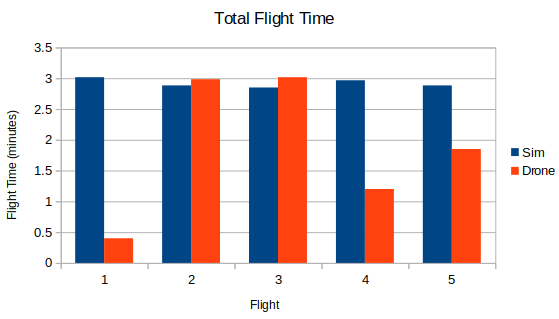
\includegraphics[width=\textwidth]{figures/Ch4/totaltimegraph.png}
	\caption{Total flight time of drone compared with that of the simulator.}
	\label{fig:totalflightgraph}
\end{figure}
\FloatBarrier

As can be seen, the simulator drone's total flight times across all five test flights are similar. On the other hand, in the real case, only flights 2 and 3 have similar flight times, as they were the only ones that the drone successfully completed the whole mission. Flight 4 was terminated prematurely to demonstrate dynamic mission input. The remaining flights suffered various malfunctions. This is further elaborated on in Section \ref{sect:reliability}. However, the two successful flights do have total time taken values that are similar to each other as well to the simulator drone's flight times. This similarity shows that there is no significant difference between a locally connected drone and a remote drone using the system developed in this study.

\section{Reliability}\label{sect:reliability}

\begin{table}[t]
  \caption{Reliability results.}
  \begin{center}
    \begin{tabular}{|c|c|}
      \hline \textbf{Flight number} & \textbf{Reliability Issues} \\ \hline \hline
      Flight 1 & Uncalibrated weight causing wrong thrust \\ \hline
      Flight 2 & Successful\\ \hline
      Flight 3 & Successful\\ \hline 
      Flight 4 & Successful but terminated\\ \hline
      Flight 5 & Depleted battery and crashed\\ \hline
    \end{tabular}
  \end{center}
  \label{table:reliability}
\end{table} 
\FloatBarrier

\begin{figure}[t]
	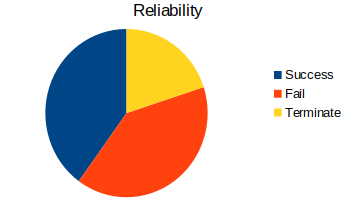
\includegraphics[width=\textwidth]{figures/Ch4/religraph.png}
	\caption{Reliability rating of the drone\textquotesingle s test flights.}
	\label{fig:religraph}
\end{figure}
\FloatBarrier

As depicted in Table \ref{table:reliability} and Figure \ref{fig:religraph}, not all the test missions were successful. Only three out of five flights were successful, showing that approximately only sixty percent of all flights will be successful with the current system.

The fourth flight is used to demonstrate a dynamic reaction to user mission input by way of a mission terminate command. Due to the premature termination in the middle of the first leg of the mission, the total flight time only amounted to less than half of the normal flight time. Currently, the user is not permitted on the web application to execute multiple missions, so mission termination is the only dynamic request available.

The test flights for the simulator drone are not listed because they are all and always will be successful regardless of battery level, weight, etc.

\section{Landing Accuracy}\label{sect:landingaccuracy}

\begin{table}[t]
  \caption{Landing accuracy results.}
  \begin{center}
    \begin{tabular}{|c|c|}
      \hline \textbf{Landing number} & \textbf{Estimated landing error margin(cm)} \\ \hline \hline
      Landing 1 & 160cm \\ \hline
      Landing 2 & 30cm\\ \hline
      Landing 3 & 90cm\\ \hline 
      Average error & 93.3cm\\ \hline 
    \end{tabular}
  \end{center}
  \label{table:landingaccuracy}
\end{table} 
\FloatBarrier

Table \ref{table:landingaccuracy} describes the results of the landing tests. The results are the differences in centimetres between the drone's original takeoff position and its landing position. The landing error offsets vary by a significant margin, implying that the GPS system alone aboard the drone is insufficient for precision landing. Therefore, the current drone will need extra modifications if it is intended to land in the drone base.

\section{Battery Consumption}\label{sect:batterylevel}
In Table \ref{table:reliability}, the last mission failed due to a depleted battery. The Pixhawk failed to detect a low voltage and did not trigger any low battery failsafe on the drone. This may be due to the large number of extra components on the drone drawing power from the battery. 

The battery on the drone proved to have enough power for approximately four complete missions. This may prove to be a major limitation in the further development and utilization of the system.

% Table~\ref{tab:hmm-based-detection-results} shows a table.

% \begin{table}[t]
%   \caption[Text shown in the LOT.]{\small Some table.}
%   \begin{center}
%     \begin{tabular}{c|c|c|c|c|c|c}
%       \hline Batch method & TP & FP & TN & FN & TPR & FPR \\ \hline \hline
%       Local ($z$-scoring) & 24 & 42 & 444 & 0 & 1 & 0.086 \\ \hline
%       Local (LRT) & 24 & 486 & 0 & 0 & 1 & 1 \\ \hline 
%       Global ($z$-scoring) & 24 & 217 & 10 & 0 & 1 & 0.956 \\ \hline 
%       Global (LRT) & 24 & 223 & 4 & 0 & 1 & 0.982 \\ \hline
%     \end{tabular}
%   \end{center}
%   \label{tab:hmm-based-detection-results}
% \end{table} 

\FloatBarrier

